% \iffalse
\let\negmedspace\undefined
\let\negthickspace\undefined
\documentclass[journal,12pt,twocolumn]{IEEEtran}
\usepackage{cite}
\usepackage{amsmath,amssymb,amsfonts,amsthm}
\usepackage{algorithmic}
\usepackage{graphicx}
\usepackage{textcomp}
\usepackage{xcolor}
\usepackage{txfonts}
\usepackage{listings}
\usepackage{enumitem}
\usepackage{mathtools}
\usepackage{gensymb}
\usepackage{comment}
\usepackage[breaklinks=true]{hyperref}
\usepackage{tkz-euclide} 
\usepackage{listings}
\usepackage{gvv}                                        
\def\inputGnumericTable{}                                 
\usepackage[latin1]{inputenc}                                
\usepackage{color}                                            
\usepackage{array}                                            
\usepackage{longtable}                                       
\usepackage{calc}                                             
\usepackage{multirow}                                         
\usepackage{hhline}                                           
\usepackage{ifthen}                                           
\usepackage{lscape}

\newtheorem{theorem}{Theorem}[section]
\newtheorem{problem}{Problem}
\newtheorem{proposition}{Proposition}[section]
\newtheorem{lemma}{Lemma}[section]
\newtheorem{corollary}[theorem]{Corollary}
\newtheorem{example}{Example}[section]
\newtheorem{definition}[problem]{Definition}
\newcommand{\BEQA}{\begin{eqnarray}}
\newcommand{\EEQA}{\end{eqnarray}}
\newcommand{\define}{\stackrel{\triangle}{=}}
\theoremstyle{remark}
\newtheorem{rem}{Remark}

\begin{document}

\bibliographystyle{IEEEtran}
\vspace{3cm}

\title{NCERT 11.9.2.3}
\author{EE23BTECH11043 - BHUVANESH SUNIL NEHETE$^{*}$% <-this % stops a space
}
\maketitle
\newpage
\bigskip

\renewcommand{\thefigure}{\theenumi}
\renewcommand{\thetable}{\theenumi}

\bibliographystyle{IEEEtran}

\section*{Question}

In an A.P. the first term is 2 and the sum of the first five terms is one-fourth of the next five terms. Show that 20\textsuperscript{th} term is $-112$.

\section*{Solution}
\begin{table}[h]
\renewcommand\thetable{1}
    \centering
    \begin{tabular}{|c|c|c|}
        \hline
        \textbf{Parameter} & \textbf{Description} & \textbf{Value}\\
        \hline
        $x(0)$ & First term & $2$\\
        \hline
        $x(19)$ & $20\textsuperscript{th}$ term & $-112$\\
        \hline
        $y(n)$ & sum upto $n\textsuperscript{th}$ term & \\
        \hline
    \end{tabular}
    \caption{Input data}
  \label{input data}
\end{table}

   \begin{align}
        x_1 + x_2 + x_3 + x_4 + x_5 = \frac{1}{4} [x_6 + x_7 + x_8 + x_9 + x_{10}]
    \end{align}
Let the common difference as \(d\)
\[[x(0) + d + x(0) + 2d + x(0) + 3d + x(0) + 4d + x(0) + 5d)] =\]
\[\frac{1}{4} [x(0) + 6d + x(0) + 7d + x(0) + 8d + x(0) + 9d + x(0) + 10d]\]

Simplifying:
    \begin{align}
        5x(0) + 15d &= \frac{1}{4}(5x(0) + 40d)\\
        20x(0) + 60d &= 5x(0) + 40d\\
        15x(0) + 20d &= 0\\
        3x(0) + 4d &= 0\\ 
        \implies x(0) &= \frac{-4d}{3}
    \end{align}

    given x(1) = x(0) + d = 2
    \begin{align}
        \implies 2 &= \frac{-4d}{3} +d\\
        \implies 2 &= \frac{-d}{3}\\
        \implies d &= -6\\
        \implies x(0) &= 8
    \end{align}
    \begin{align}
        x(20)&=x(0)+20d\\
        &=8+20(-6) = -112
    \end{align}
\centering
$x(0) = 8\quad \text{and}\quad d = -6$
    \begin{align}
        x(n)&=x(0)+nd\\
        \implies x(n)&=8+(n)(-6)\\
        \implies x(n)&=8-6n
    \end{align}    
The Z-transform of a sequence $x(n)$ is given by:
    \begin{align}
        X(z) = \sum_{n=0}^{\infty} x(n) z^{-n} 
    \end{align}
For the sequence $x_n = 8 - 6n$ when $n > 0$, we can write:
    \begin{align}
        X(z) = \sum_{n=1}^{\infty} (8 - 6n)z^{-n}\\
        X(z) = \sum_{n=1}^{\infty} 8z^{-n} - \sum_{n=1}^{\infty} 6nz^{-n}\\
        X(z) = 8U(z) + 6(-z)\frac{d}{dz} U(z)\\
        X(z)=\frac{8}{1-z^{-1}}+\frac{6z^{-1}}{(1-z^{-1})^{2}}
    \end{align}\
The function $f(n) = 8 - 6n$ using step function is defined as follows:
    \begin{figure}[h]
        \centering
        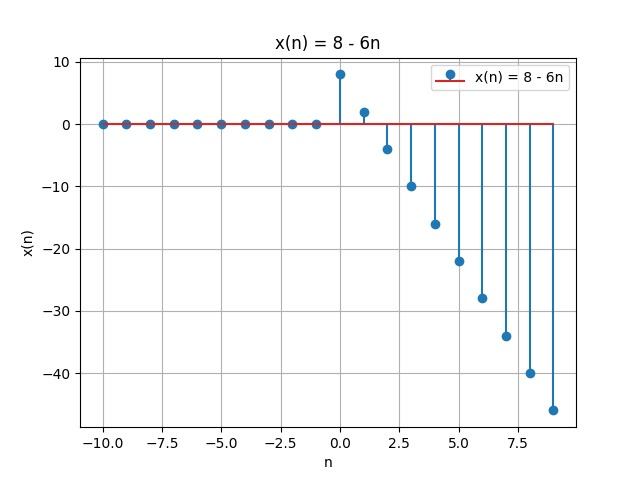
\includegraphics[width=0.95\linewidth]{figs/Figure_1.png}
        \caption{graph of x(n) = 8 - 6n}
        \label{8 - 6n dicrete function}
    \end{figure}
    \begin{align}
        x(n) = 
        \begin{cases}
            8 - 6n, & \text{if } n \geq 0 \\
            0, & \text{if } n < 0
        \end{cases}
    \end{align}

Given that \( n > 0 \)
\[\therefore ROC : |z| > 1\]
    
\end{document}
